\section{Manifestation}



\fonction{Création}
Le logiciel dispose d'un assistant permettant de se configurer facilement pour une nouvelle manifestation.

Les données sont par la suite entièrement modifiables.



\section{Orgas}



\fonction{Inscription}
Les orgas peuvent insérer leurs propres informations dans le système lors de l'inscription, et pouvoir les modifier plus tard.

Les orgas peuvent effectuer ces opérations à l'aide d'une interface web, accessible en ligne.

\fonction{Authentification}
Les orgas peuvent accéder à leurs données et les modifier de manière sécurisée, qu'ils soient ou non étudiants à l'INSA de Lyon.

Il est préférable que les étudiants de l'INSA s'authentifient à l'aide du système CAS.

\fonction{Disponibilités}
Les orgas peuvent déclarer plusieurs plages horaires pendant lesquelles ils peuvent travailler.

\fonction{Amis}
Les orgas peuvent indiquer les personnes avec lesquelles ils souhaitent travailler. Ces souhaits doivent être respectés dans la mesure du possible.

\fonction{Édition de badges}
L'\oh{} peut imprimer des badges pour les orgas.

Les informations pouvant être portées sur les badges sont les suivantes, et doivent être totalement adaptables : 
\begin{itemize}
\item Nom de l'orga
\item Catégorie de l'orga
\end{itemize}

Un visuel peut être ajouté et personnalisé.


\fonction{Importation/Exportation}
La liste des orgas, à laquelle on peut ajouter les différentes informations conçernant les orgas, peut être exportée vers et importées depuis un format de fichier standard.


\subsection{Lettres d'excuses aux départements}
\fonction{Génération et impression}
Le logiciel permet de générer et d'imprimer des lettres d'excuses adressées aux directeurs des départements.

\fonction{Personnalisation}
Les éléments suivants peuvent être ajoutés et modifiés aux lettres d'excuse : 
\begin{itemize}
 \item Nom, adresse, et logotype de l'association
\item Nom et signature du président de l'association.
\item Département et année de l'orga excusé
\item Nom et adresse du destinataire
\item Date
\end{itemize}


\fonction{Administration des orgas}
L' \oh{} peut modifier les informations concernant un orga.


\subsection{Catégories d'orgas}
\fonction{Création}
L'\oh{} peut créer un nombre illimité de catégories d'orgas.

\fonction{Assignation des orgas}
Les orgas peuvent se déclarer comme membre d'une catégorie d'orgas, cette affectation devient active après validation de l'\oh{}. Un orga peut appartenir à plusieurs catégories, certaines peuvent être cachées.

\section{Tâches}

\begin{figure}[h!t]
\centering
\includegraphics[width=\textwidth]{process-tachessvg.png}
\label{fig:ptaches}
\caption{Processus de création et de validation d'un groupe de tâches.}
\end{figure}


\fonction{Création}
Un orga peut créer un nombre illimité de tâches.

\fonction{Validation}
Une tâche peut être validée par le chef de l'équipe à laquelle se rapporte la tâche ou par un \oh{}.

Cette validation doit s'effectuer selon le processus décrit dans la figure \ref{fig:ptaches}

\fonction{Commentaires}
Un nombre illimité de commentaires peuvent être ajoutés à une tâche par différents orgas humains.


\fonction{Importation/Exportation}
Les tâches (et notamment leurs description) peuvent être exportées vers et importées depuis un format de fichier standard.


\subsection{Groupe de tâches}
\fonction{Inclusion de tâches}
Une tâche est nécessairement incluse dans un groupe de tâches.
\fonction{Création}
Un orga peut créer un groupe de tâches directement lors de la création d'une nouvelle tâche.

\fonction{Commentaires}
Un nombre illimité de commentaires peuvent être ajoutés à un groupe de tâches par différents orgas humains.

\section{Lieux}
\fonction{Création}
Un orga peut créer un lieu directement lors de la création d'une nouvelle tâche.

\fonction{Affichage}
Le logiciel peut générer, et imprimer les états suivants :
\begin{itemize}
 \item Carte globale des lieux
\item Liste des lieux avec mini-carte
\end{itemize}
On tolérera un simple export des lieux vers le logiciel Google Earth\textregistered{}.

\section{Matériel}

\fonction{Création}
Un orga peut créer un matériel directement lors de la création d'une nouvelle tâche.

\fonction{Besoins en Matériel}
L'\oh{} peut générer, visualiser et imprimer la quantité totale de matériel nécessaire, heure par heure.

\fonction{Planning}
L'\oh{} peut générer, visualiser et imprimer le planning d'un matériel.

\section{Créneaux}

\begin{figure}[h!t]
\centering
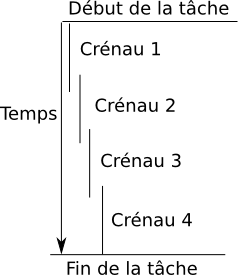
\includegraphics[width=.3\textwidth]{tache-crenaux.png}

\caption{Décomposition d'une tâche en créneaux.}
\label{fig:crenaux}
\end{figure}



\fonction{Création}
Le logiciel peut créer automatiquement des créneaux pour une tâche. Cf figure \ref{fig:crenaux}

\fonction{Planification automatique}
Le logiciel peut assigner automatiquement des créneaux aux orgas.

\fonction{Planification assistée}
Le logiciel permet de gérer manuellement les assignations de créneaux, en aidant au maximum l'utilisateur dans ses choix.

\fonction{Résultats à produire}
Le logiciel peut générer et afficher les états suivants : 

\begin{itemize}
\item Nombre de créneaux assignés, restant à assigner et orgas disponibles en fonction du temps.
\item Liste des créneaux, triés et groupés indifférament par : 	\begin{itemize}
								  \item Orga
								  \item Équipe
								  \item Horaire
\item Heure
								 \end{itemize}
\item Liste des orgas, triés et groupés indifférament par :  	\begin{itemize}
								  \item Catégorie
								  \item Équipe
								  \item Département
								 \end{itemize}
\item Groupé par tâche, et pour chaque créneau, le lieu du créneau suivant et précédent de l'orga affecté.

\end{itemize}

\fonction{Vérification des erreurs}
Le logiciel affiche une rapport détaillé lorsque une incohérence est détectée dans les créneaux (temps trop court entre deux créneaux, manque d'orgas pour un créneau, tâche sans créneaux, trop peu de temps pour dormir)



\fonction{Affichage à l'écran}
Le logiciel permet un affichage intéractif des résultats produits, un exemple est présenté dans la figure \ref{fig:interactivite}

\begin{figure}[h!t]
\centering
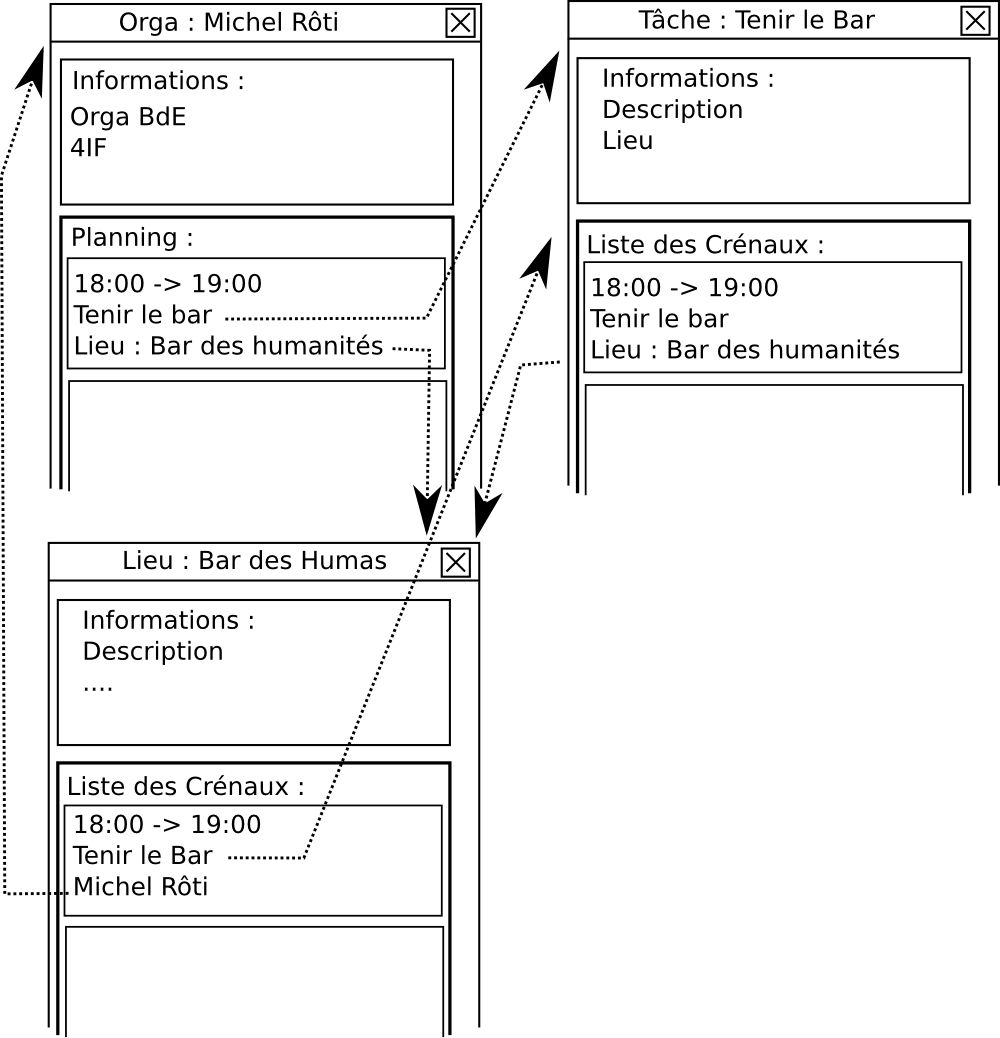
\includegraphics[width=\textwidth]{interactivite.png}

Un clic sur une information ouvre la fenêtre indiquée par la flèche en pointillés..
\caption{Démonstration de l'interactivité}
\label{fig:interactivite}
\end{figure}


\fonction{Affichage de type agenda}
Le logiciel permet d'afficher de manière interactive, sur un affichage de type agenda, la liste des créneaux pour une tâche. Il est possible de faire coincider cet affichage avec l'heure actuelle.
Cf figure \ref{fig:agenda}

\begin{figure}[h!t]
\centering
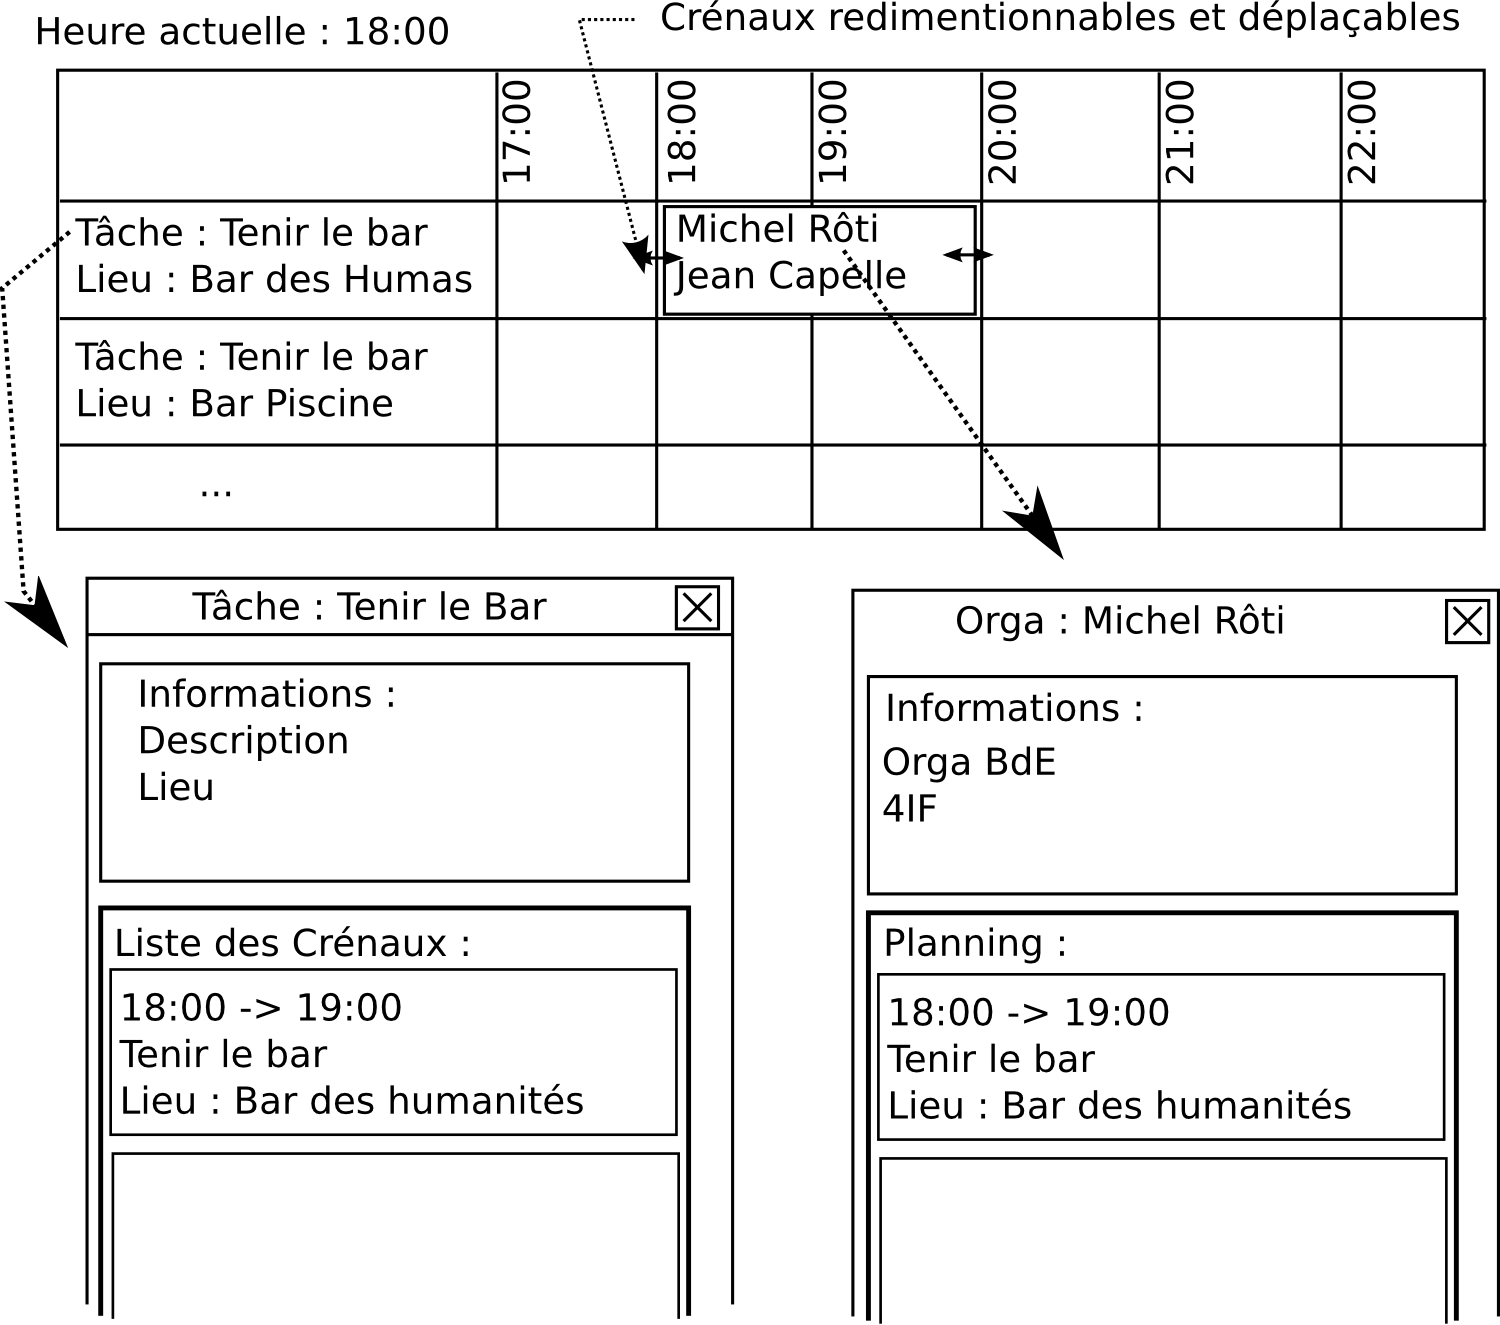
\includegraphics[width=\textwidth]{vue-agenda.png}

\caption{Vue interactive de type agenda}
\label{fig:agenda}
\end{figure}


\fonction{Impression}
Le logiciel peut produire et imprimer tous les résultats produits sous forme adaptée à l'impression, y compris la vue de type agenda.

\fonction{Format des plannings}

Notamment pour les plannings orga, il est possible de personnaliser de manière complète le format des plannings. On peut notamment choisir :
\begin{itemize}
 \item La présentation de chaque créneau (nature et disposition des informations à afficher)
\item Les informations présentées en en-tête, pied de page
\item Les informations présentées à la première et dernière page
\item Les informations présentées au recto du planning (plan de la manifestation par exemple)
\end{itemize}

\section{Véhicule}

\fonction{Création}
Les orgas peuvent créer un nombre illimité de voyages.


\fonction{Contrôle d'erreurs}
Le logiciel signale à l'utilisateur si un véhicule affecté à une tâche n'est pas présent au lieu de la tâche.





\section{Voyages}

\fonction{Création}
Les orgas peuvent créer un nombre illimité de voyages.

\fonction{Planification automatique}
Le logiciel peut assigner automatiquement des créneaux aux orgas.

\fonction{Contrôle de capacité maximale}
Le logiciel signale à l'utilisateur si un véhicule affecté doit transporter plus que sa capacité.

\subsection{Résultats à produire}
Le logiciel peut générer, afficher de manière interactive et imprimer :
\fonction{Fiche de véhicule ``Véhicule Book''}
Une fiche de véhicule qui indique, pour un véhicule, la liste de ses voyages et toutes les informations qui leurs sont associées, en particulier le matériel à charger.

Pour chaque voyage, un aperçu du trajet peut être donné sous forme de carte.

\fonction{Fiches de transport}
Une fiche de coffre qui indique pour chaque voyage d'un véhicule la liste du matériel et des orgas à transporter.
En en-tête figure les informations spécifiques au voyage et au véhicule.

